% \PassOptionsToPackage{quiet}{fontspec}
\documentclass[12pt,a4paper,UTF8]{article}
\usepackage{thesis} % 格式控制
\usepackage{indentfirst}
\usepackage{dirtree}  % 添加这一行
\setlength{\parindent}{2em} % 控制首行缩进  
\addtolength{\parskip}{3pt} % 控制段落距离  
\onehalfspacing % 1.5倍行距  
\graphicspath{{./figures/}} % 指定图片所在文件夹  


\classname{统计与大数据分析}  % 设置课程名称
\makepagestyle{深度学习部分}{统计与大数据分析 ~额外工作}




\begin{document}
\maketitlepage{Classify Leaves}{西1-210}{樊铧纬}{3220104373}{\today}{肖朦} %封面页 

\maketoc    %目录页
\section{实验目的和要求}
\begin{problem}
The task is predicting categories of leaf images. This dataset contains 176 categories, 18353 training images, 8800 test images. Each category has at least 50 images for training. The test set is split evenly into the public and private leaderboard.

The evaluation metric for this competition is Classification Accuracy.
\end{problem}



\section{数据集}

\texttt{train.csv}: the training set
\texttt{test.csv}: the test set
\texttt{sample\_submission.csv}: a sample submission file in the correct format (the labels are randomly generated so the initial accuracy is roughly 1/176)
\texttt{images/}: the folder contains all images


\textbf{Data fields:}
\texttt{image}: the image path, such as\texttt{ images/0.jpg}
\texttt{label}: the category name

使用pandas库的常见功能,我们可以查看数据集的基本信息。


数据集基本信息:
\begin{itemize}
    \item 总样本数: 18353
    \item 总类别数: 176
\end{itemize}

样本数最多的前10个类别:
\begin{itemize}
    \item \texttt{maclura\_pomifera}: 353个样本
    \item \texttt{ulmus\_rubra}: 235个样本
    \item \texttt{prunus\_virginiana}: 223个样本
    \item \texttt{acer\_rubrum}: 217个样本
    \item \texttt{broussonettia\_papyrifera}: 214个样本
    \item \texttt{prunus\_sargentii}: 209个样本
    \item \texttt{ptelea\_trifoliata}: 193个样本
    \item \texttt{ulmus\_pumila}: 189个样本
    \item \texttt{abies\_concolor}: 176个样本
    \item \texttt{asimina\_triloba}: 174个样本
\end{itemize}

样本数最少的前10个类别:
\begin{itemize}
    \item \texttt{aesculus\_flava}: 68个样本
    \item \texttt{betula\_lenta}: 68个样本
    \item \texttt{pinus\_thunbergii}: 67个样本
    \item \texttt{acer\_griseum}: 64个样本
    \item \texttt{ailanthus\_altissima}: 58个样本
    \item \texttt{cedrus\_deodara}: 58个样本
    \item \texttt{ulmus\_procera}: 58个样本
    \item \texttt{crataegus\_crus-galli}: 54个样本
    \item \texttt{evodia\_daniellii}: 53个样本
    \item \texttt{juniperus\_virginiana}: 51个样本
\end{itemize}

类别分布统计:
\begin{itemize}
    \item 平均每类样本数: 104.28
    \item 最大样本数: 353
    \item 最小样本数: 51
    \item 样本数标准差: 38.67
\end{itemize}


\begin{table}[htbp]
    \centering
    \begin{tabular}{lrr}
        \hline
        & image & label \\
        \hline
        count & 18353 & 18353 \\
        unique & 18353 & 176 \\
        top & images/18352.jpg & maclura\_pomifera \\
        freq & 1 & 353 \\
        \hline
    \end{tabular}
    \caption{数据集基本统计信息}
    \label{tab:dataset-stats}
\end{table}

\section{训练过程与结果}

这次训练我租用了Autodl平台的两张3090显卡进行训练,使用pytorch框架,使用AdamW优化器,使用交叉熵损失函数,使用余弦退火学习率调度器,使用early stopping防止过拟合。

\begin{table}[htbp]
  \centering
  \resizebox{\columnwidth}{!}{%
  \begin{tabular}{|c|c|c|c|}
  \hline
  \textbf{Method}                                          & \textbf{Epoch} & \textbf{Private Score} & \textbf{Public Score} \\ \hline
  resnet18   Naive                                         & 50             & 0.79522                & 0.79886               \\ \hline
  resnet18 with   trick                                    & 50             & 0.95181                & 0.94977               \\ \hline
  resnet18.a1\_in1k                                        & 50             & 0.94909                & 0.9484                \\ \hline
  resnet50d                                                & 90             & 0.88568                & 0.88363               \\ \hline
  resnet50d                                                & 30             & 0.92204                & 0.92113               \\ \hline
  resnet50d                                                & 48             & 0.96181                & 0.96022               \\ \hline
  \textbf{resnet50d}                                       & \textbf{50}    & \textbf{0.9659}        & \textbf{0.9625}       \\ \hline
  mixnet\_xl                                               & 50             & 0.96977                & 0.9634                \\ \hline
  inception\_resnet\_v2 label smoothing                    & 50             & 0.96909                & 0.96204               \\ \hline
  \textbf{inception\_resnet\_v2.tf\_ens\_adv\_in1k}        & \textbf{50}    & \textbf{0.97181}       & \textbf{0.96727}      \\ \hline
  tf\_mobilenetv3\_small\_minimal\_100.in1k                & 50             & 0.93022                & 0.92727               \\ \hline
  mobilenetv2\_100.ra\_in1k                                & 50             & 0.96113                & 0.95659               \\ \hline
  resnet101.a1h\_in1k                                      & 33             & 0.96113                & 0.95886               \\ \hline
  \textbf{resnet101.a1h\_in1k}                             & \textbf{44}    & \textbf{0.9709}        & \textbf{0.96863}      \\ \hline
  resnext                                                  & 50             & 0.93318                & 0.93                  \\ \hline
  seresnext50\_32x4d.racm\_in1k                            & 20             & 0.95636                & 0.95409               \\ \hline
  seresnext50\_32x4d.racm\_in1k                            & 33             & 0.9659                 & 0.96113               \\ \hline
  seresnext50\_32x4d.racm\_in1k                            & 42             & 0.96863                & 0.96636               \\ \hline
  seresnext50\_32x4d.racm\_in1k                            & 50             & 0.96954                & 0.9675                \\ \hline
  \textbf{seresnext50\_32x4d.racm\_in1k   with finetuning} & \textbf{45}    & \textbf{0.98204}       & \textbf{0.97886}      \\ \hline
  \textbf{seresnext50\_32x4d.racm\_in1k   with finetuning} & \textbf{50}    & \textbf{0.9834}        & \textbf{0.97795}      \\ \hline
  选择使用正确率低的分类重新训练小模型                                       & /              & 0.8834                 & 0.8859                \\ \hline
  5个96分学习器进行bagging集成,投票法                                  & /              & 0.9659                 & 0.9625                \\ \hline
  \textbf{4个97分学习器进行bagging集成,投票法}                         & \textbf{/}     & \textbf{0.98704}       & \textbf{0.98545}      \\ \hline
  \end{tabular}%
  }
  \caption{训练过程与结果}
  \end{table}


\begin{figure}[htbp] \centering 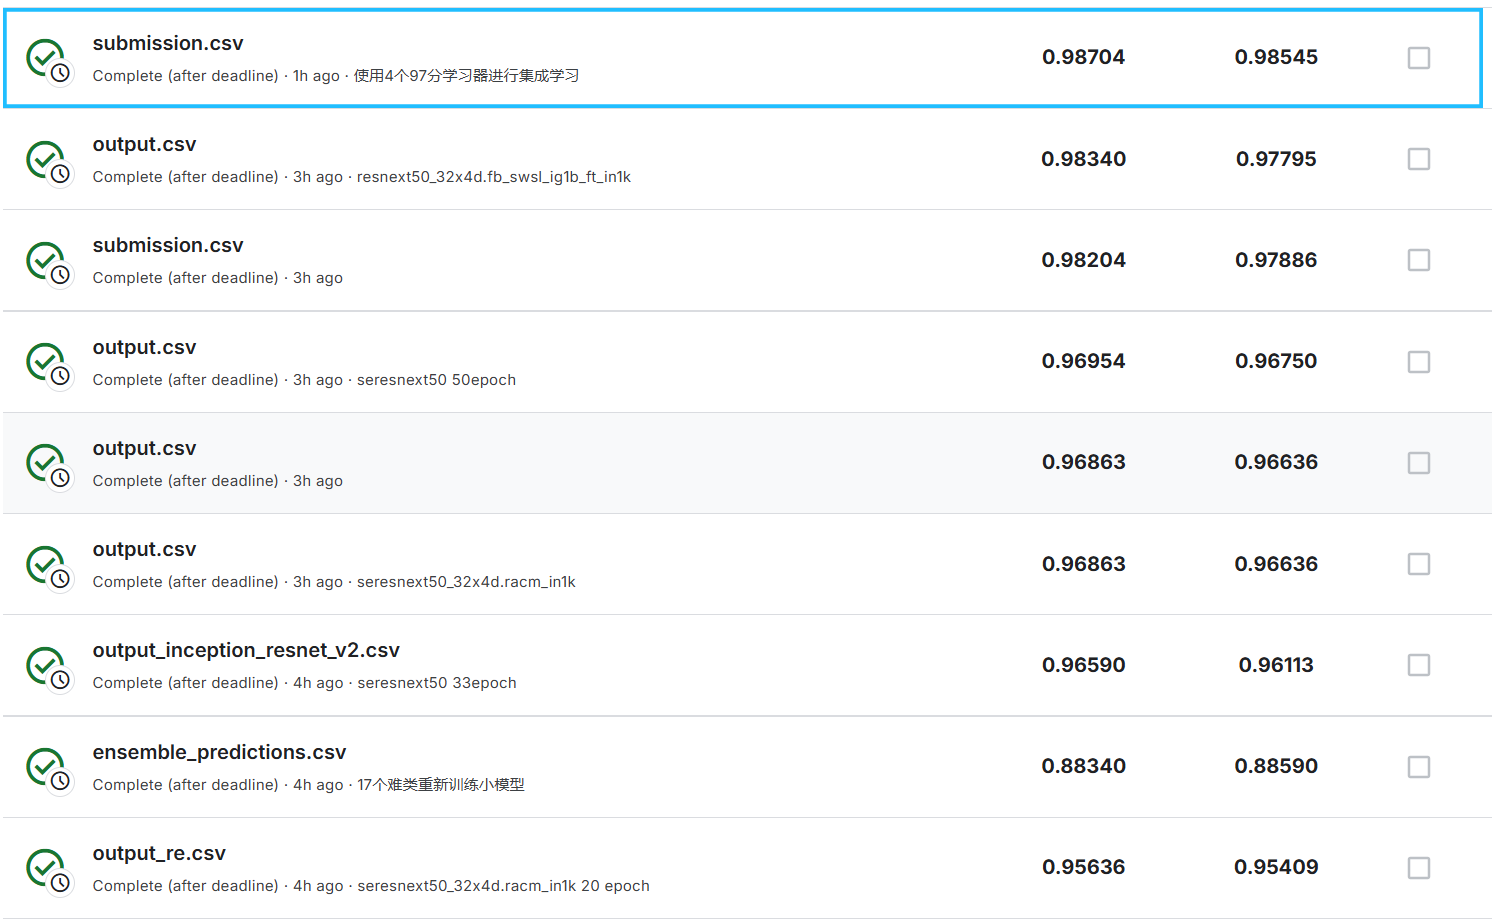
\includegraphics[width=0.7\textwidth]{figures/2024-12-12-18-42-21.png} \caption{ Kaggle平台截图} \end{figure}

\begin{figure}[htbp] \centering 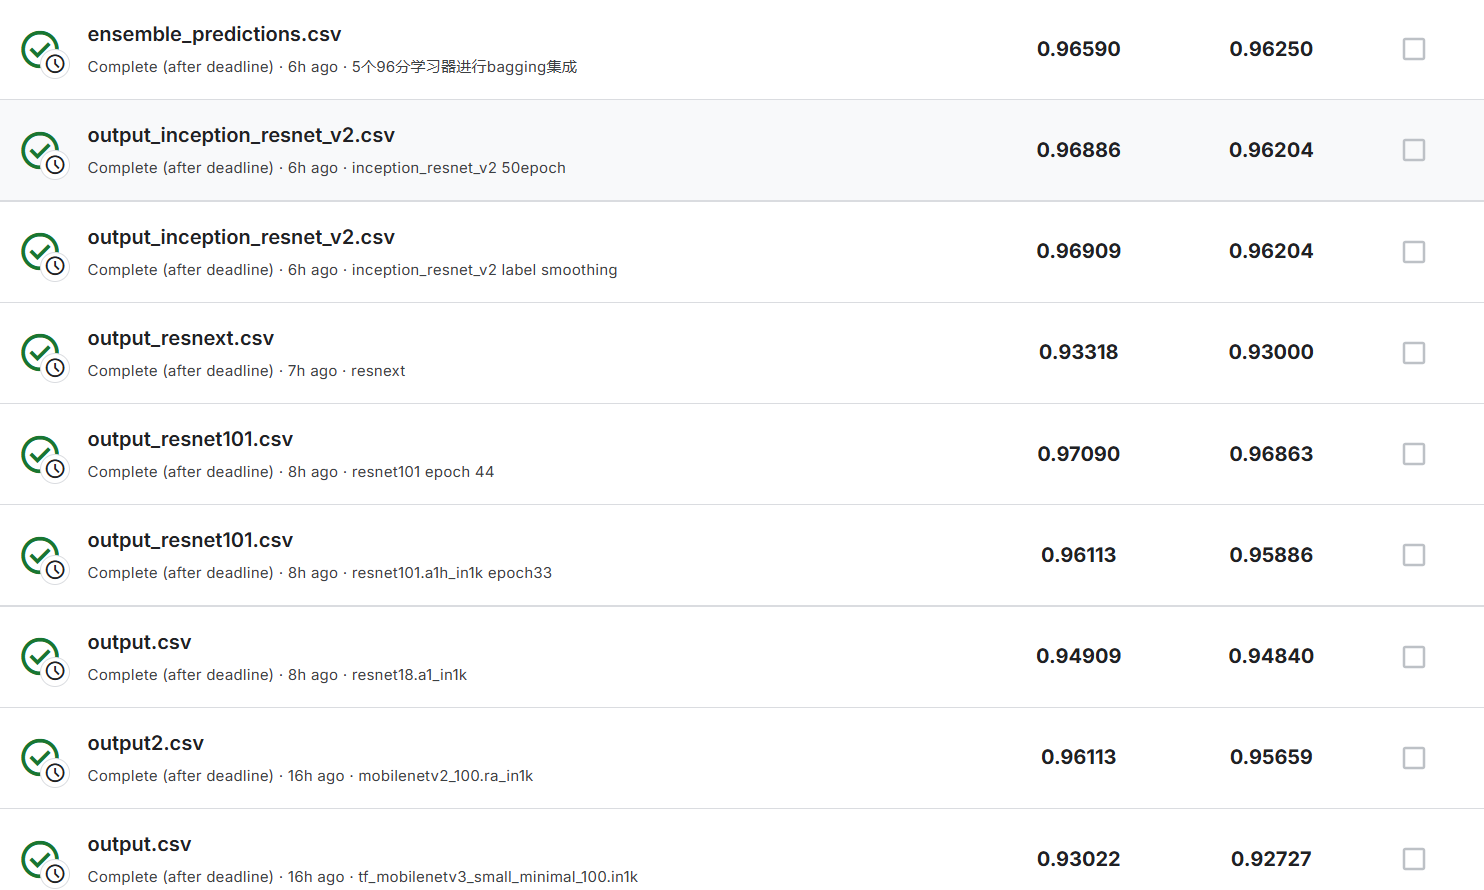
\includegraphics[width=0.7\textwidth]{figures/2024-12-12-18-42-44.png} \caption{ Kaggle平台截图} \end{figure}

\begin{figure}[htbp] \centering 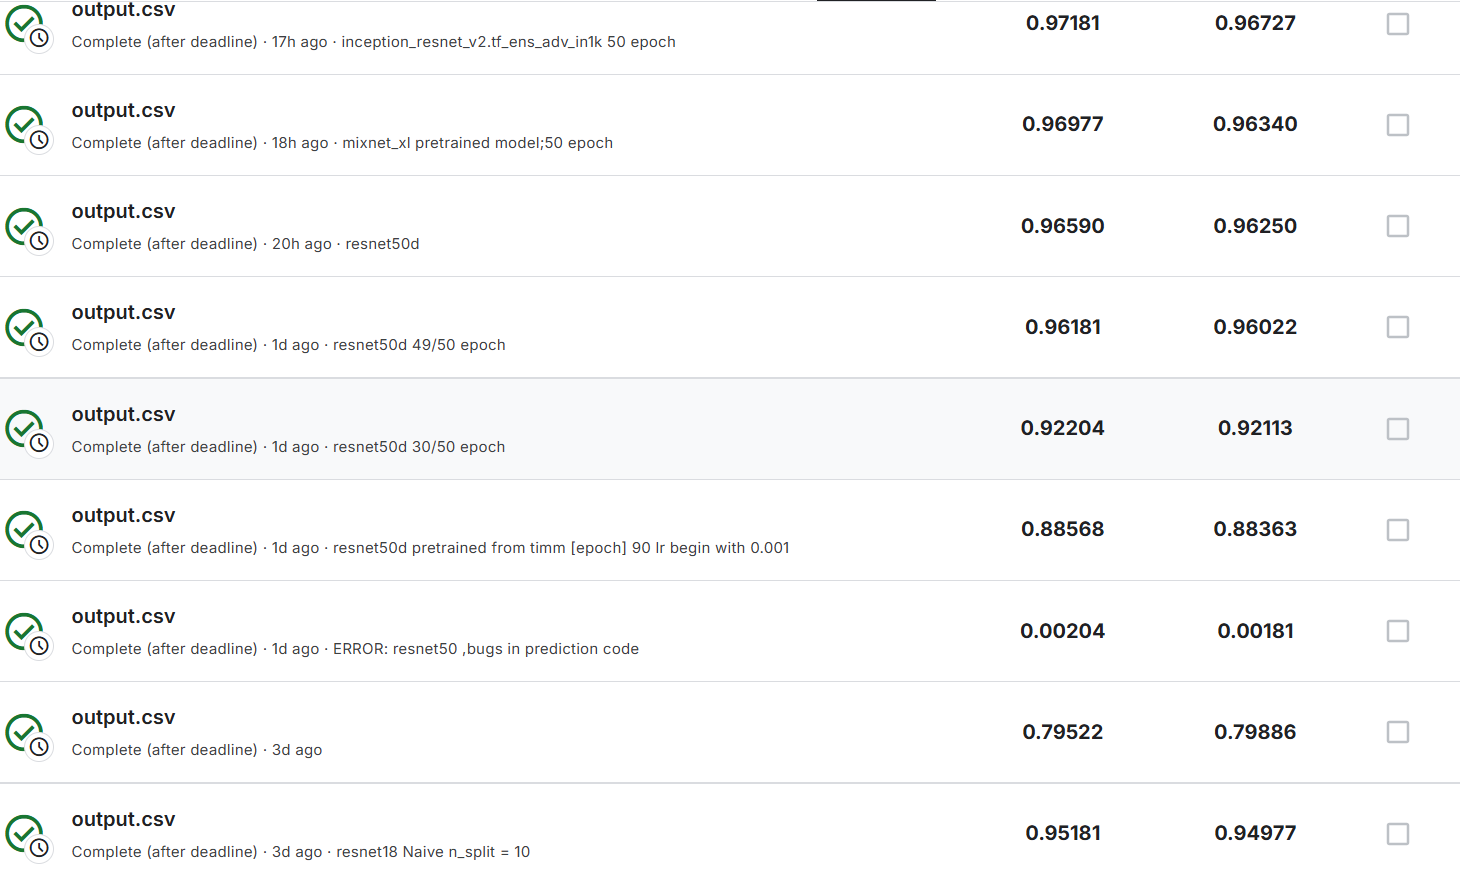
\includegraphics[width=0.7\textwidth]{figures/2024-12-12-18-43-13.png} \caption{ Kaggle平台截图 }\end{figure}

\section{准备阶段}


\begin{lstlisting}[language=Python, caption=查看显卡信息]
gpustat
\end{lstlisting}

\begin{lstlisting}[language=Python, caption=把图片分文件夹放好]
import os
import shutil
import pandas as pd
import argparse

# 添加命令行参数解析
def parse_args():
    parser = argparse.ArgumentParser(description='整理图片到训练和测试目录')
    parser.add_argument('root_dir', type=str, help='项目根目录的路径')
    return parser.parse_args()

# 全局变量现在需要通过函数来设置
def get_output_dirs(root_dir):
    return {
        'train': os.path.join(root_dir, 'img_train'),
        'test': os.path.join(root_dir, 'img_test')
    }

def setup_directories(dirs):
    """创建必要的输出目录"""
    for directory in dirs.values():
        if not os.path.exists(directory):
            os.makedirs(directory)

def process_train_images(dirs, train_csv_path='train.csv'):
    """处理训练集图片"""
    print("开始处理训练集图片...")
    
    df_train = pd.read_csv(train_csv_path)
    
    labels = df_train['label'].unique()
    for label in labels:
        label_dir = os.path.join(dirs['train'], label)
        if not os.path.exists(label_dir):
            os.makedirs(label_dir)
    
    for index, row in df_train.iterrows():
        src = row['image']
        dst = os.path.join(dirs['train'], row['label'], os.path.basename(src))
        
        try:
            shutil.copy2(src, dst)
            print(f"复制 {src} 到 {dst}")
        except FileNotFoundError:
            print(f"警告: 找不到文件 {src}")
        except Exception as e:
            print(f"复制 {src} 时发生错误: {str(e)}")
    
    print("训练集图片整理完成!")

def process_test_images(dirs, test_csv_path='test.csv'):
    """处理测试集图片"""
    print("\n开始处理测试集图片...")
    
    df_test = pd.read_csv(test_csv_path)
    test_images = df_test['image'].tolist()
    
    for img_path in test_images:
        try:
            src = img_path
            dst = os.path.join(dirs['test'], os.path.basename(img_path))
            
            shutil.copy2(src, dst)
            print(f"复制 {src} 到 {dst}")
        except FileNotFoundError:
            print(f"警告: 找不到文件 {src}")
        except Exception as e:
            print(f"复制 {src} 时发生错误: {str(e)}")
    
    print("测试集图片整理完成!")

def main():
    """主函数"""
    args = parse_args()
    output_dirs = get_output_dirs(args.root_dir)
    
    setup_directories(output_dirs)
    process_train_images(output_dirs)
    process_test_images(output_dirs)

if __name__ == "__main__":
    main() 
\end{lstlisting}


\begin{lstlisting}[language=Python]
train_df.describe() 
\end{lstlisting}

\clearpage

\section{第一阶段——自己搭建网络}
这个数据集是李沐老师《动手学深度学习》课程中的一个数据集,正好之前也看过这门课程前面的一些内容,所以最开始的时候,我打算自己搭建一个网络,然后使用这个数据集进行训练。

\begin{lstlisting}[language=Python, caption=残差神经网络的Baseline]
class Residual(nn.Module):
  def __init__(self, input_channels, num_channels, use_1x1conv=False, strides=1):
      super().__init__()
      self.conv1 = nn.Conv2d(input_channels, num_channels,
                            kernel_size=3, padding=1, stride=strides)
      self.conv2 = nn.Conv2d(num_channels, num_channels,
                            kernel_size=3, padding=1)
      if use_1x1conv:
          self.conv3 = nn.Conv2d(input_channels, num_channels,
                                kernel_size=1, stride=strides)
      else:
          self.conv3 = None
      self.bn1 = nn.BatchNorm2d(num_channels)
      self.bn2 = nn.BatchNorm2d(num_channels)

  def forward(self, X):
      Y = F.relu(self.bn1(self.conv1(X)))
      Y = self.bn2(self.conv2(Y))
      if self.conv3:
          X = self.conv3(X)
      Y += X
      return F.relu(Y)

class CustomResNet(nn.Module):
  def __init__(self, num_classes=10):
      super().__init__()
      # 修改第一层以接受3通道RGB图像
      self.b1 = nn.Sequential(
          nn.Conv2d(3, 64, kernel_size=7, stride=2, padding=3),
          nn.BatchNorm2d(64), 
          nn.ReLU(),
          nn.Dropout(0.1),
          nn.MaxPool2d(kernel_size=3, stride=2, padding=1)
      )
      
      # 构建残差块
      self.b2 = self._make_layer(64, 64, 2, first_block=True)
      self.b3 = self._make_layer(64, 128, 2)
      self.b4 = self._make_layer(128, 256, 2)
      self.b5 = self._make_layer(256, 512, 2)
      
      self.avgpool = nn.AdaptiveAvgPool2d((1, 1))
      self.flatten = nn.Flatten()
      self.dropout = nn.Dropout(0.5)
      self.fc = nn.Linear(512, num_classes)

  def _make_layer(self, input_channels, num_channels, num_residuals, first_block=False):
      layers = []
      for i in range(num_residuals):
          if i == 0 and not first_block:
              layers.append(Residual(input_channels, num_channels, use_1x1conv=True, strides=2))
          else:
              layers.append(Residual(num_channels, num_channels))
      return nn.Sequential(*layers)

  def forward(self, x):
      x = self.b1(x)
      x = self.b2(x)
      x = self.b3(x)
      x = self.b4(x)
      x = self.b5(x)
      x = self.avgpool(x)
      x = self.flatten(x)
      x = self.dropout(x)
      x = self.fc(x)
      return x
\end{lstlisting}


\begin{lstlisting}[language=Python, caption=训练代码]
# 创建模型
model = CustomResNet(num_classes=num_classes)
model = model.to(device)

# 定义损失函数和优化器
criterion = nn.CrossEntropyLoss()
# 使用SGD优化器替代Adam
# optimizer = torch.optim.SGD(model.parameters(), lr=learning_rate, momentum=0.9, weight_decay=5e-4)
optimizer = torch.optim.Adam(model.parameters(), lr=learning_rate)
# 添加学习率调度器
scheduler = torch.optim.lr_scheduler.CosineAnnealingLR(optimizer, T_max=num_epochs)

# 记录最佳验证准确率和对应的模型路径
best_val_acc = 0.0
best_model_path = None

# 初始化记录列表
train_losses = []
train_accs = []
val_losses = []
val_accs = []

# 训练循环
for epoch in range(num_epochs):
    model.train()
    epoch_train_loss = 0
    train_correct = 0
    train_total = 0
    
    # 训练阶段
    train_pbar = tqdm(train_loader, desc=f'Epoch [{epoch+1}/{num_epochs}] 训练')
    for images, labels in train_pbar:
        images, labels = images.to(device), labels.to(device)
        
        optimizer.zero_grad()
        outputs = model(images)
        loss = criterion(outputs, labels)
        loss.backward()
        optimizer.step()
        
        epoch_train_loss += loss.item()
        _, predicted = outputs.max(1)
        train_total += labels.size(0)
        train_correct += predicted.eq(labels).sum().item()
        
        train_pbar.set_postfix({
            'loss': f'{epoch_train_loss/train_total:.4f}',
            'acc': f'{100.*train_correct/train_total:.2f}%'
        })
    
    # 计算训练集平均损失和准确率
    epoch_train_loss = epoch_train_loss / len(train_loader)
    epoch_train_acc = 100. * train_correct / train_total
    
    # 验证阶段
    model.eval()
    epoch_val_loss = 0
    val_correct = 0
    val_total = 0
    
    val_pbar = tqdm(val_loader, desc='验证中')
    with torch.no_grad():
        for images, labels in val_pbar:
            images, labels = images.to(device), labels.to(device)
            outputs = model(images)
            loss = criterion(outputs, labels)
            
            epoch_val_loss += loss.item()
            _, predicted = outputs.max(1)
            val_total += labels.size(0)
            val_correct += predicted.eq(labels).sum().item()
            
            val_pbar.set_postfix({
                'loss': f'{epoch_val_loss/val_total:.4f}',
                'acc': f'{100.*val_correct/val_total:.2f}%'
            })
    
    # 计算验证集平均损失和准确率
    epoch_val_loss = epoch_val_loss / len(val_loader)
    epoch_val_acc = 100. * val_correct / val_total
    
    # 记录损失和准确率
    train_losses.append(epoch_train_loss)
    train_accs.append(epoch_train_acc)
    val_losses.append(epoch_val_loss)
    val_accs.append(epoch_val_acc)
    
    # 只在验证准确率更高时保存最佳模型
    if epoch_val_acc > best_val_acc:
        # 如果已存在之前的最佳模型文件,则删除它
        if best_model_path and os.path.exists(best_model_path):
            os.remove(best_model_path)
        
        best_val_acc = epoch_val_acc
        best_model_path = os.path.join(save_dir, f'best_model_acc_{epoch_val_acc:.2f}.pth')
        torch.save({
            'epoch': epoch + 1,
            'model_state_dict': model.state_dict(),
            'optimizer_state_dict': optimizer.state_dict(),
            'val_accuracy': epoch_val_acc,
            'train_loss': epoch_train_loss,
            'val_loss': epoch_val_loss
        }, best_model_path)
        print(f'保存最佳模型到: {best_model_path}')
    
    # 绘制并保存训练曲线
    plot_training_curves(
        train_losses, train_accs, 
        val_losses, val_accs,
        save_dir, 'training_curves'
    )
    
    print(f'Epoch [{epoch+1}/{num_epochs}]')
    print(f'训练损失: {epoch_train_loss:.4f}, 训练准确率: {epoch_train_acc:.2f}%')
    print(f'验证损失: {epoch_val_loss:.4f}, 验证准确率: {epoch_val_acc:.2f}%')
    print('--------------------')
    
    # 更新学习率
    scheduler.step()
\end{lstlisting}

这份代码里面是有一个bug
\begin{figure}[htbp] \centering 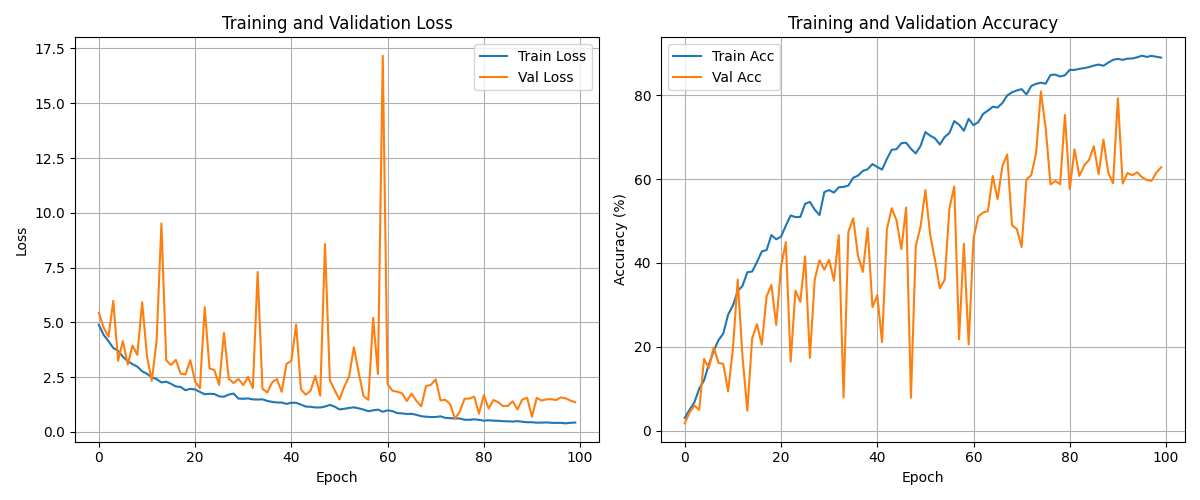
\includegraphics[width=0.7\textwidth]{figures/2024-12-12-19-27-16.png} \caption{第一次训练曲线} \end{figure}


这份代码在lr=0.001,batch\_size=64,num\_epochs=100,save\_dir="./checkpoints"的配置下,训练了50个epoch,验证集的准确率达到了85.5\%左右。

为了后续的实验,我需要将这份代码封装成一个函数,方便后续的实验。

所以我将这份代码的不同部分拆成了不同的py文件。

详见我的代码。

\begin{figure}[htbp] \centering 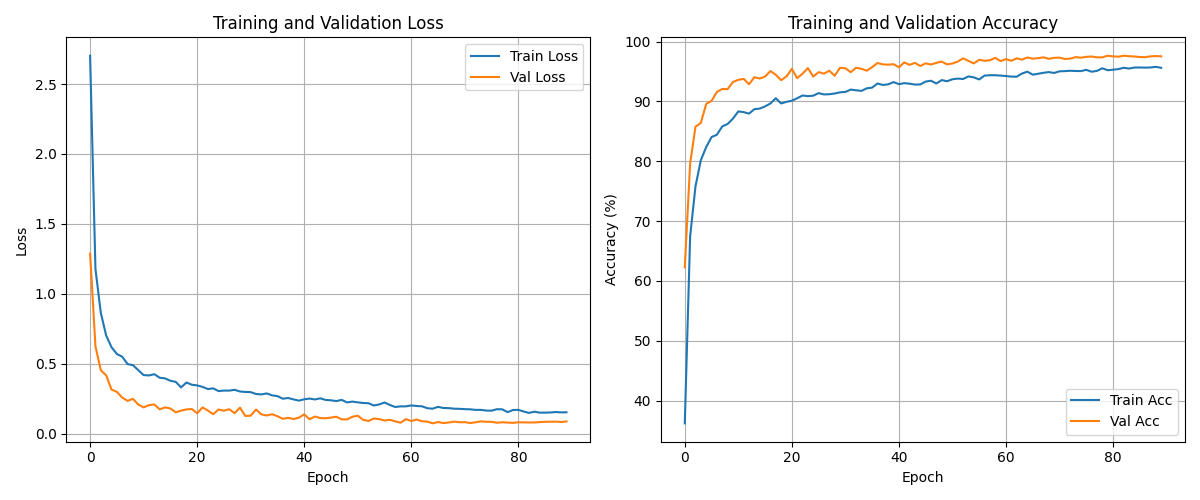
\includegraphics[width=0.7\textwidth]{figures/2024-12-12-19-27-42.png} \caption{resnet50d训练} \end{figure}



\subsection{增加label smoothing}
标签平滑(Label Smoothing)是一种正则化技术,用于防止模型过度自信。它通过将原始的one-hot标签转换为软标签来实现。

具体来说,对于一个K类分类问题:
- 传统的one-hot标签:正确类别为1,其他类别为0
- 标签平滑后:正确类别为1-α,其他类别为α/(K-1),其中α是平滑系数

标签平滑的优点:
\begin{itemize}
    \item 防止模型过度自信,提高泛化能力
    \item 增加模型的鲁棒性
    \item 缓解过拟合问题
\end{itemize}

在这个实验中,使用了标签平滑技术,平滑系数设为0.1。这意味着:
\begin{itemize}
    \item 正确类别的标签值从1变为0.9
    \item 其他类别的标签值从0变为0.1/175 (因为总共有176个类别)
\end{itemize}


\begin{lstlisting}[language=Python, caption=增加label smoothing]
  class LabelSmoothingLoss(nn.Module):
  """
  标签平滑损失函数
  
  参数:
      smoothing (float): 平滑因子,默认0.1表示使用0.1的平滑系数
  """
  def __init__(self, smoothing=0.1):
      super().__init__()
      self.confidence = 1.0 - smoothing
      self.smoothing = smoothing

  def forward(self, x: torch.Tensor, target: torch.Tensor) -> torch.Tensor:
      """
      计算平滑后的损失值
      
      参数:
          x (torch.Tensor): 模型输出的logits
          target (torch.Tensor): 目标标签
          
      返回:
          torch.Tensor: 计算得到的损失值
      """
      logprobs = F.log_softmax(x, dim=-1)
      nll_loss = -logprobs.gather(dim=-1, index=target.unsqueeze(1))
      nll_loss = nll_loss.squeeze(1)
      smooth_loss = -logprobs.mean(dim=-1)
      loss = self.confidence * nll_loss + self.smoothing * smooth_loss
      return loss.mean()

def create_criterion(name="crossentropy", smoothing=0.1):
  """
  创建损失函数
  
  参数:
      name: 损失函数名称,支持 'crossentropy' 和 'labelsmoothing'
      smoothing: 标签平滑系数,仅在使用labelsmoothing时有效
      
  返回:
      nn.Module: 损失函数
  """
  if name.lower() == "crossentropy":
      return nn.CrossEntropyLoss()
  elif name.lower() == "labelsmoothing":
      return LabelSmoothingLoss(smoothing=smoothing)
  else:
      raise NotImplementedError(f"Loss function {name} not implemented")
\end{lstlisting}
\subsection{不同层使用不同的学习率}


\begin{itemize}
    \item \textbf{针对性训练}: 对于预训练模型的微调,通常最后几层需要更大的学习率以适应新任务,而前面的层保持较小的学习率以保留预训练的特征
    \item \textbf{提高训练效率}: 通过为不同层设置合适的学习率,可以加快模型收敛速度
    \item \textbf{防止过拟合}: 较小的学习率可以防止底层特征提取器过度适应新数据集
    \item \textbf{平衡迁移学习}: 在迁移学习中,这种策略可以很好地平衡预训练知识的保留和新任务的适应
\end{itemize}

在本实验中,我们对全连接层使用了10倍于其他层的学习率,这是因为全连接层需要从头开始学习新的分类任务,而其他层主要是微调预训练的特征。

\begin{lstlisting}[language=Python, caption=不同层使用不同的学习率]
optimizer = torch.optim.AdamW([{'params': params},
    {'params': model.fc.parameters(),
        'lr': args.lr * 10}],
    lr=args.lr, weight_decay=2e-4)

scheduler = torch.optim.lr_scheduler.CosineAnnealingLR(
optimizer, T_max=args.epochs, eta_min=args.lr/20
)
\end{lstlisting}


\subsection{k-fold}

使用StratifiedKFold对数据集进行分层,然后进行k-fold交叉验证,详见训练记录


k-fold交叉验证是一种评估机器学习模型性能的方法。它将数据集分成k个相等大小的子集,每次使用k-1个子集作为训练集,剩下的1个子集作为验证集。这个过程重复k次,每个子集都会作为一次验证集。

在本实验中,我使用了StratifiedKFold进行5折交叉验证。StratifiedKFold是k-fold的一个变体,它在划分数据时会\textbf{保持每个类别的样本比例},这对于不平衡的数据集特别有用。

k-fold交叉验证的主要优点包括:

\begin{itemize}
    \item 充分利用有限的数据,每个样本都会被用作训练和验证
    \item 得到更可靠的模型性能评估
    \item 减少过拟合的风险
    \item 评估模型的稳定性
\end{itemize}

具体实现时,我使用了sklearn库中的StratifiedKFold类:

\begin{lstlisting}[language=Python]
from sklearn.model_selection import StratifiedKFold

skf = StratifiedKFold(n_splits=5, shuffle=True, random_state=42)
for fold, (train_idx, val_idx) in enumerate(skf.split(X, y)):
    train_data = dataset[train_idx]
    val_data = dataset[val_idx]
    # 训练模型...
\end{lstlisting}

\clearpage
\section{第二阶段——使用预训练模型进行fine tuning}
由于第一阶段训练的模型效果并不理想,所以第二阶段我打算使用预训练模型进行fine tuning。

首先我尝试了pytorch的nn库自带的预训练模型进行训练,详见训练记录

\begin{figure}[htbp] \centering 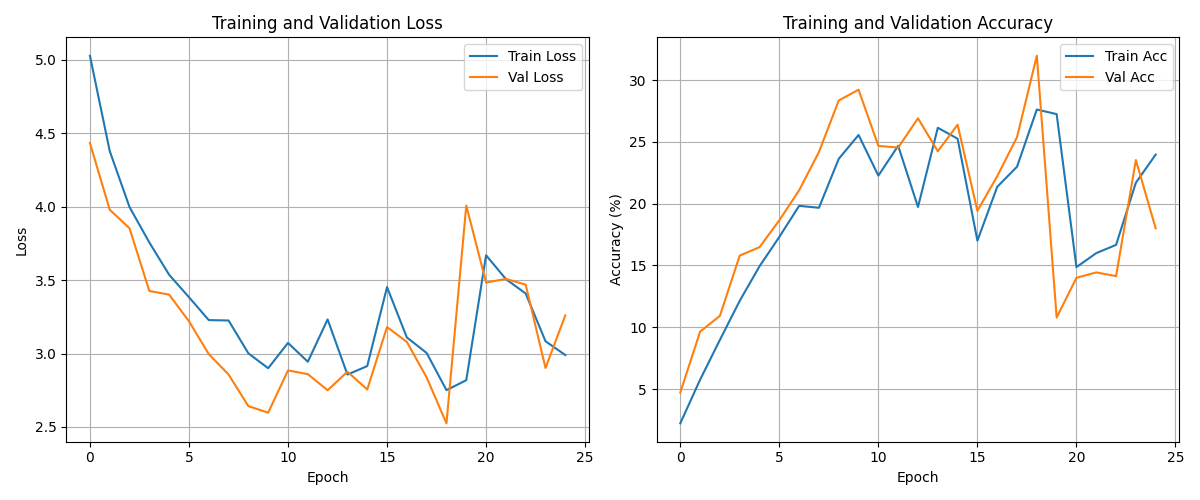
\includegraphics[width=0.7\textwidth]{figures/2024-12-12-19-29-03.png} \caption{vit训练失败,v2e训练显存不够} \end{figure}


\subsection{使用vit和v2e模型}
在实验中,我也尝试使用了vit和v2e模型,但是由于显卡的显存不够,训练时长已经超过了我的预算范围,所以只能放弃,希望之后可以有机会拿到更好的卡,进行实验。

vit由于代码有一些bug,训练了20个epoch左右,系统正确率一直在20\%左右徘徊,中途我结束了训练

\subsection{使用timm库进行训练}

这里需要注意的是,因为我的显卡没有办法连接外网,所以pretrained的模型需要我手动下载,放到本地


timm库是一个开源的深度学习库,全称为PyTorch Image Models,它提供了大量的预训练模型和训练工具。主要特点包括:

\begin{itemize}
    \item 提供了超过500个预训练模型,包括ResNet、VGG、Inception等经典模型
    \item 支持多种数据增强方法和训练技巧
    \item 提供了模型训练和评估的工具函数
    \item 支持模型导出和部署
    \item 与PyTorch生态系统完全兼容
\end{itemize}

在本次实验中,我主要使用了timm库提供的预训练模型进行迁移学习。由于显卡无法连接外网,我需要手动下载预训练模型权重文件并放到本地。

使用timm库的主要步骤如下:
\begin{enumerate}
    \item 使用\texttt{timm.create\_model()}创建模型
    \item 加载预训练权重
    \item 修改最后的全连接层以适应本任务的类别数
    \item 进行模型训练
\end{enumerate}

\begin{lstlisting}[language=Python, caption=使用timm库进行训练,核心代码]
model = timm.create_model('inception_resnet_v2.tf_ens_adv_in1k',pretrained=False)
model.load_state_dict(torch.load('result/mixnet_xl/pytorch_model.bin', map_location=device))
model.fc = nn.Linear(model.num_features, num_classes)
print(model.fc.in_features)
nn.init.xavier_uniform_(model.fc.weight)
model.cuda()
\end{lstlisting}

\begin{figure}[htbp] \centering 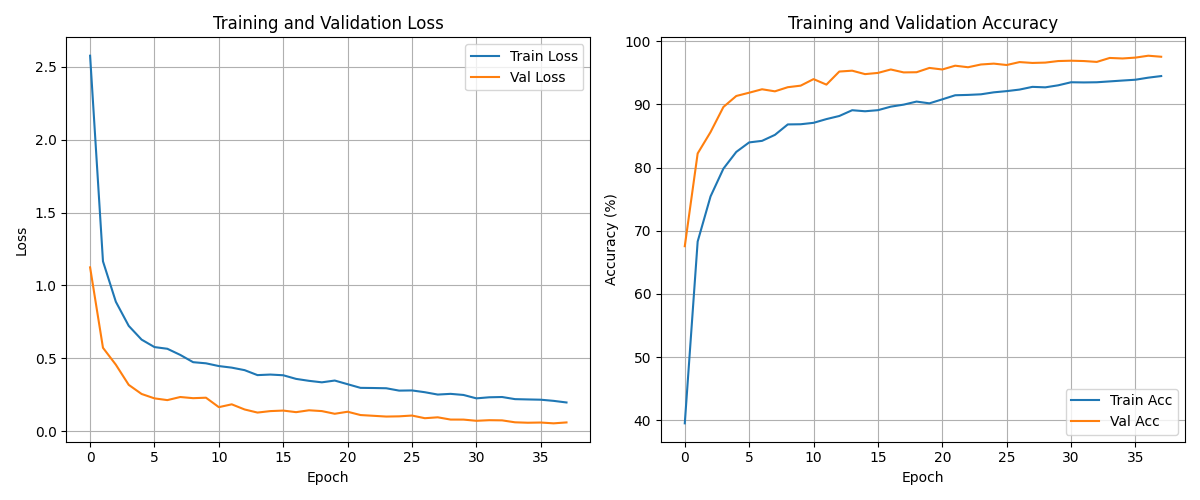
\includegraphics[width=0.8\textwidth]{figures/2024-12-12-19-28-14.png} \caption{mixnet\_xl score = 0.969} \end{figure}

\begin{figure}[htbp] \centering 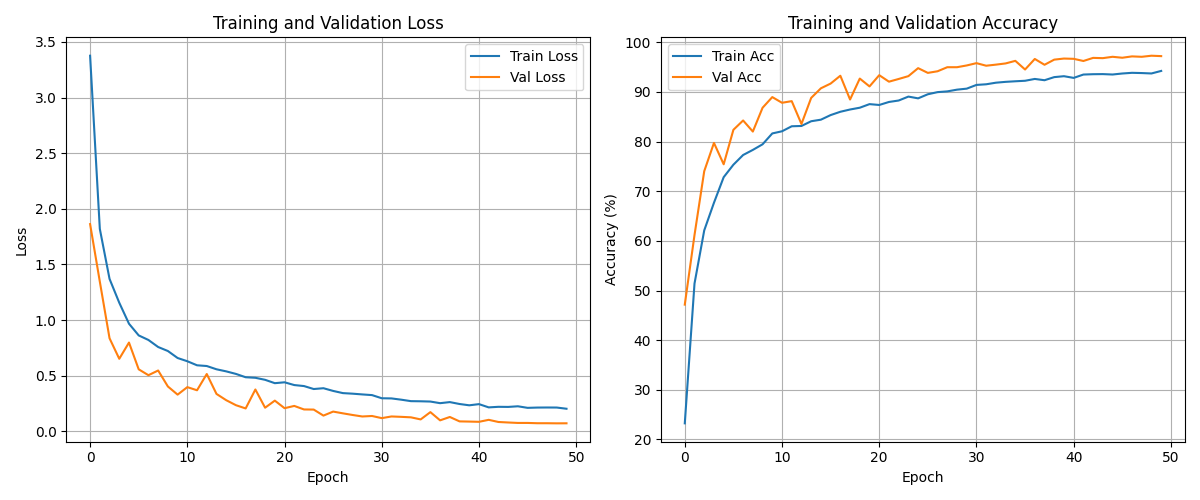
\includegraphics[width=0.8\textwidth]{figures/2024-12-12-19-28-41.png} \caption{inception\_resnet\_v2.tf\_ens\_adv\_in1k score 97.181} \end{figure}

\begin{figure}[htbp] \centering 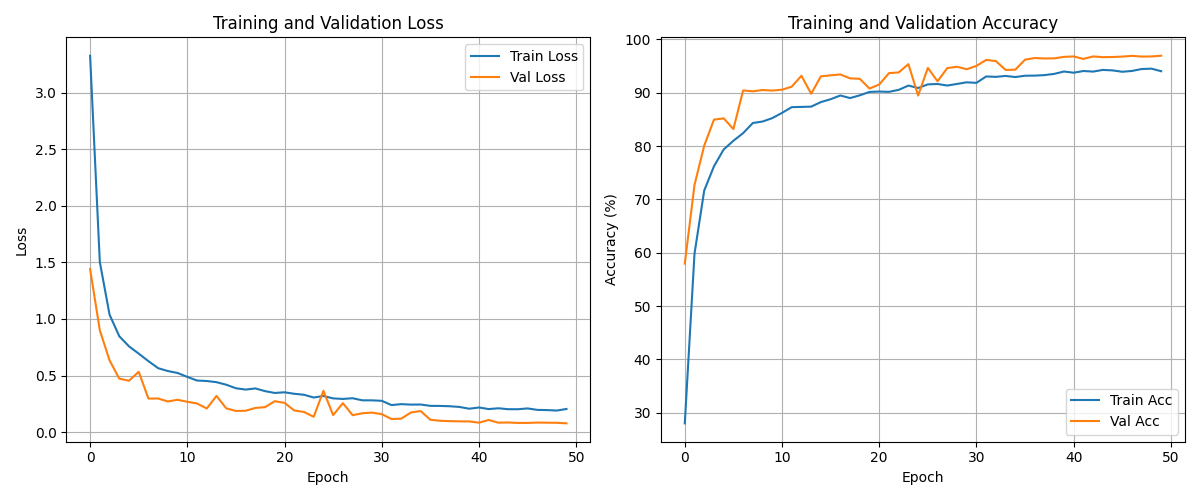
\includegraphics[width=0.8\textwidth]{figures/2024-12-12-19-29-39.png} \caption{mobilenetv2\_100.ra\_in1k.bin score=96.133} \end{figure}


\begin{figure}[htbp] \centering 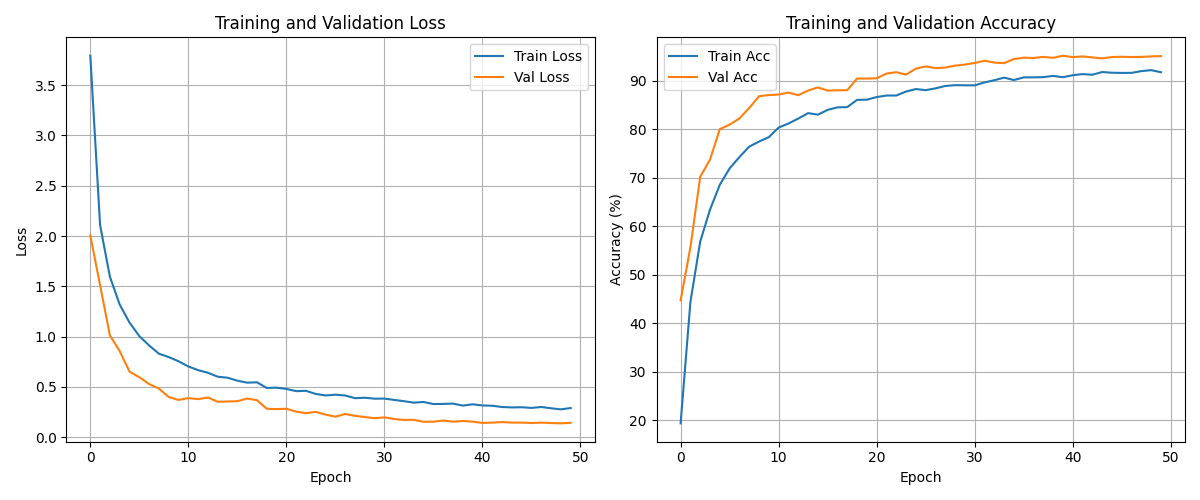
\includegraphics[width=0.8\textwidth]{figures/2024-12-12-19-30-02.png} \caption{tf\_mobilenetv3\_small\_minimal\_100.in1k score=93.022} \end{figure}


\begin{figure}[htbp] \centering 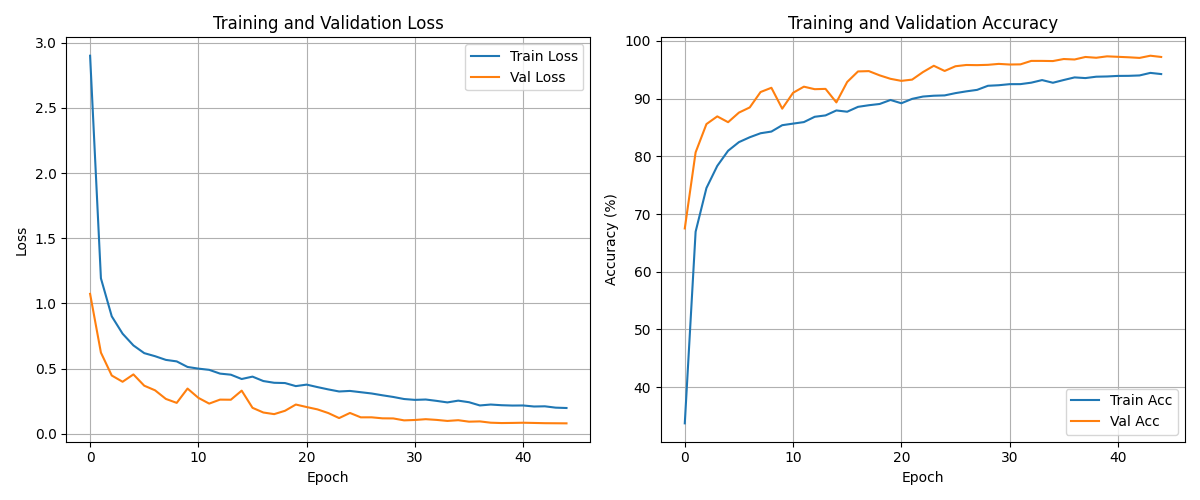
\includegraphics[width=0.8\textwidth]{figures/2024-12-12-19-30-41.png} \caption{resnet101.a1\_in1k epoch 33: score = 96.133 epoch 50: score = 97.090} \end{figure}


后续还有一些图片,由于比较类似,所以就不放了

\clearpage
\section{第三阶段——集成学习}

这次实验我也尝试使用了集成学习进行训练。

首先我使用了当时使用\texttt{inception\_resnet\_v2.tf\_ens\_adv\_in1k}模型训练出的97的模型进行统计,发现有一些分类正确率比较低,所以把这些小分类抽出来,单独训练了一个数据集。

但是训练的结果并不好。反而比单独的模型分数低了。

\begin{lstlisting}[language=Python, caption=使用前后两个模型进行训练]
model2.fc = nn.Linear(model2.num_features, 17)
model2.load_state_dict( torch.load('result/20241212_143856/0_best_model.pth', map_location=device)['state_dict'])
model2 = model2.to(device)
model2.eval()
\end{lstlisting}

所以使用了bagging的方法,采用简单投票法进行实验。

最开始我使用5个96分左右的学习器进行预测,最后的分数并不高,没有超过97


后来我调整了我的图像预处理,使用数据增强,使用dropout,使用label smoothing后,训练出了4个97分左右的学习器,使用这四个97分的学习器进行预测,最后的分数超过了98.


后续调整了batchsize继续训练,给4个模型按照原始分数给予不同的权重,最后分数达到了98.

\section{感受}

这次实验是在自学深度学习的课程的时候突发奇想开始做的,肖老师讲的ML给我打开了一扇新世界的大门,在自学的过程中遇到了很多困难,包括用云服务器也花了一点点零花钱qwq

我深刻感受到了调参的不易,以及数据集的重要性。

有些时候,花了很多时间加了很多trick,分数不增反降,我也意识到,对于深度学习模型,我需要学习的内容还有很多。

通过这次实践的训练,我更加了解了pytorch进行训练的基础步骤,以及timm和huggingface的使用,更重要的是我积累了一些使用服务器和显卡进行训练的经验,这对后续的研究很有帮助。有关使用服务器和pytorch的笔记,我记录在了\href{https://www.philfan.cn/Robotics/Environment/System-server/#_13}{个人网站}上面

\end{document}
